\documentclass[14pt]{beamer}
\usepackage[utf8]{inputenc}
\usepackage[T1]{fontenc}
\usepackage{lmodern}
\usepackage[english]{babel}
\usepackage{graphicx}
\usetheme{Boadilla}

\makeatletter
\def\verbatim{\small\@verbatim \frenchspacing\@vobeyspaces \@xverbatim}
\makeatother


\begin{document}
	\author{Lukáš Růžička}
	\title{Zlatý slavík, Karel GIT}
	%\subtitle{}
	%\logo{}
%	\institute{Red Hat}
	\date{Fall 2020}
	%\subject{}
	%\setbeamercovered{transparent}
	%\setbeamertemplate{navigation symbols}{}
	\begin{frame}[plain]
		\maketitle
	\end{frame}


	\begin{frame}{Co je GIT?}
	\begin{itemize}
		\item verzovací systém
		\item open source
		\item s aktivním vývojem
		\item vytvořil je Linus Torvalds
		\item distribuovaný (necentralizovaný)
	\end{itemize}
	\end{frame}


	\begin{frame}{Proč?}
	 Vytváření věcí duševní povahy často zahrnuje:
		\vspace{5pt}
		
	\begin{itemize}
		\item přepisování
		\item mazání
		\item zkoušení slepých cest
		\item návraty k předchozímu
		\item revize a korekce od spolupracovníků
	\end{itemize}
\end{frame}
		
\begin{frame}{Srovnání s kdysi}
	
	\begin{tabular}{l|l}
		\textbf{pravěk} & \textbf{gitvěk} \\
		\hline opište si zadání &  fork \\
		průběžně odevzdávejte & git commit \\
		zkus ještě další verzi & git branch \\
		použij obě verze, přepiš  & git merge \\
		tady jsou opravy, přepiš & git merge \\
		raději bych přece jen tu dřívější verzi & git reset \\
		zahoď to & git rm \\
        cos to zahodil, ty jelito? & git clone
	\end{tabular}
	
	\vspace{10pt}
		
	Prostě $\ldots${} \textbf{Vždycky GIT!}

\end{frame}

\begin{frame}{Co potřebujeme?}
	\begin{itemize}
		\item účet na nějakém serveru s gitem
		\item nainstalovaný git
	\end{itemize}
\end{frame}

	\begin{frame}{Úkol 1 - Přípravné práce}
		\begin{itemize}
		\item Fedora: sudo dnf install git
		\item Debian: sudo apt-get install git
		\item Mac: http://git-scm.com/download/mac
		\item Windows: http://git-scm.com/download/win
		\item github.com -- založit účet
		\end{itemize}
	\end{frame}

	\begin{frame}{Konfigurace gitu}
		\begin{itemize}
		\item \texttt{git config -\,-global user.name "Your Name"}
		\item \texttt{git config -\,-global user.email "yourname@example.com"}
		\end{itemize}
	\end{frame}

	\begin{frame}{Vytváříme první repozitář}
		\begin{enumerate}
		\item Běžte na stránku svého profilu.
		\item Klikněte na \textbf{Repositories}.
		\item Klikněte na \textbf{New}.
		\item Vyplňte údaje.
		\item Klikněte na \textbf{Create repository}.
		\end{enumerate}
	\end{frame}

	\begin{frame}{Stránka profilu}
        \begin{center}
        \frame{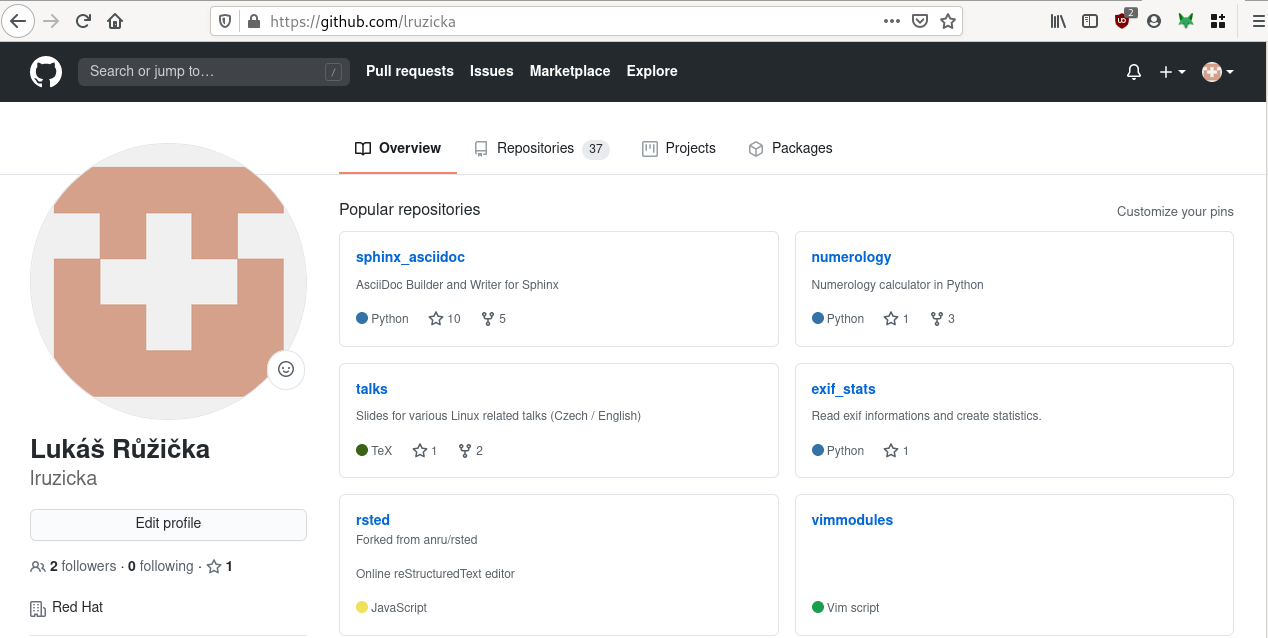
\includegraphics[width=10cm]{images/profil.png}}
        \end{center}
	\end{frame}

	\begin{frame}{Nový repozitář}
	\begin{center}
		\frame{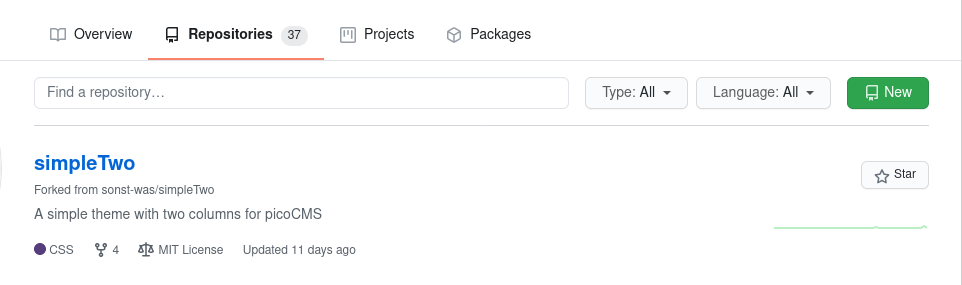
\includegraphics[width=10cm]{images/repositories.png}}
	\end{center}
	\end{frame}

	\begin{frame}{Vytvořit nový repozitář}
	\begin{center}
		\frame{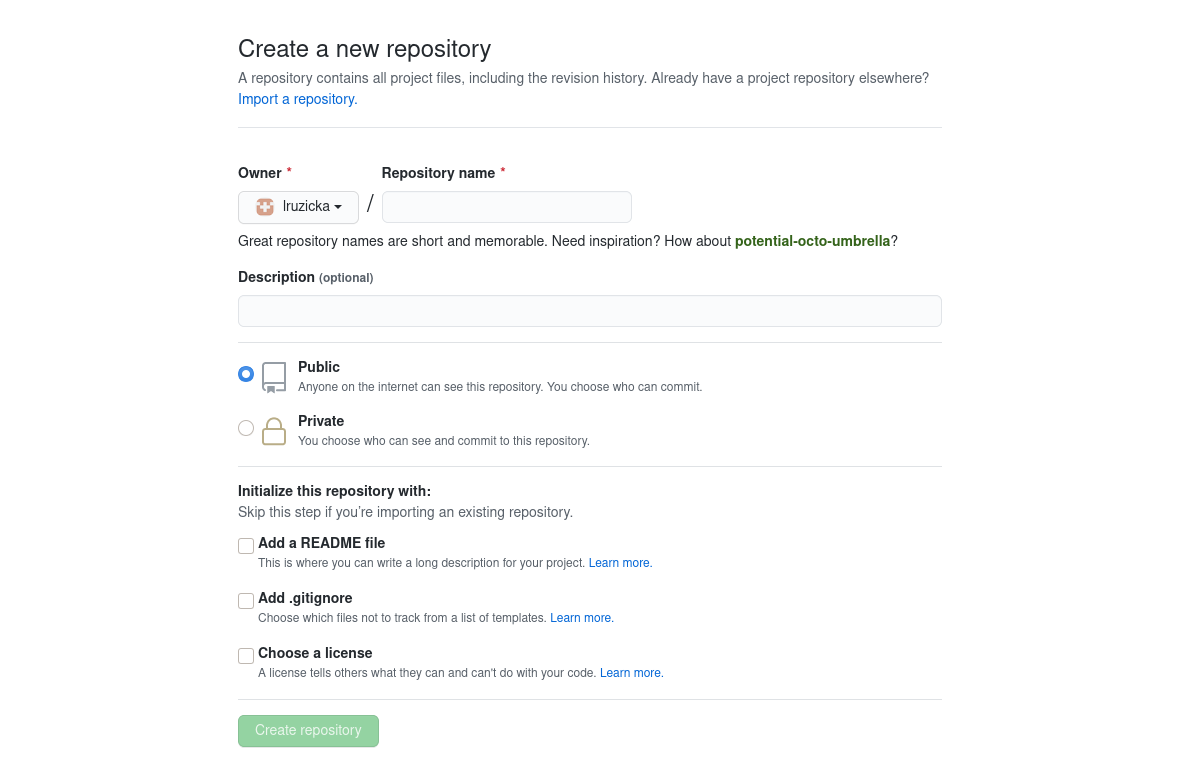
\includegraphics[width=10cm]{images/createnew.png}}
	\end{center}
	\end{frame}

	\begin{frame}{Konfigurace gitu}
	\begin{itemize}
		\item \texttt{git config -\,-global user.name "Your Name"}
		\item \texttt{git config -\,-global user.email "yourname@example.com"}
	\end{itemize}
	\end{frame}


	\begin{frame}{Plán úkolů před}
		\begin{enumerate}
		\item Založit účet.
		\item Nainstalovat git.
	\end{enumerate}
	\end{frame}

	\begin{frame}{Plán úkolů github.}
		\begin{enumerate}
			\item Vytvořit nové repo s README.
			\item Nastavit github.io.
			\item Naklonovat toto repo. (git clone)
		\end{enumerate}
	\end{frame}
	
	\begin{frame}{Plán úkolů -- první kroky}
	\begin{enumerate}
		\item Upravit README.
		\item Přidat úpravy ne server.
		\item git status
		\item git add
		\item git commit
		\item git push
		\item git log
	\end{enumerate}
   Několikrát opakovat pro vytvoření commit historie.
	\end{frame}

	\begin{frame}{Plán úkolů -- vývoj oddělený od produkce}
	\begin{enumerate}
		\item Vytvořit novou větev a pokračovat vývoj tam.
		\item git checkout (-b)
		\item git push -\,-set-upstream origin branch
		\item git branch
		\item git branch -d (-D)
		\item git push -d origin branch
	\end{enumerate}
	Několikrát opakovat pro vytvoření commit historie.
	\end{frame}

	\begin{frame}{Plán úkolů -- upravujeme commit historii}
		\begin{enumerate}
			\item git rebase -i
			\item git push -\,-force
		\end{enumerate}
	\end{frame}
	

	\begin{frame}{Plán úkolů -- zveřejnění vývoje}
		\begin{enumerate}
			\item Vzít obsah vývojové větve do produkční.
			\item git merge
			\item git rebase
		\end{enumerate}
	\end{frame}

	\begin{frame}{Plán úkolů -- řešíme konflikt}
		\begin{enumerate}
			\item Dvě větve s vývojem (master, develop).
			\item řešení konfliktu
			\item merge
		\end{enumerate}
	\end{frame}

	\begin{frame}{Plán úkolů -- návrat k původnímu}
	\begin{enumerate}
		\item Vracíme se k dřívější verzi.
		\item REFs
		\item git revert
		\item git reset (soft, hard)
		\item git checkout <commit>
	\end{enumerate}
	\end{frame}

	\begin{frame}{Plán úkolů -- zachraňujeme, co se dá}
		\begin{enumerate}
			\item Hledání ztraceného času
			\item git reflog
			\item detached state
		\end{enumerate}
	\end{frame}

	\begin{frame}{Plán úkolů -- úkládáme na později}
	\begin{enumerate}
		\item Uložit pro strýčka Příhodu
		\item git stash
	\end{enumerate}
	\end{frame}

	
	\begin{frame}{Tree and Branches}
    \begin{center}
%	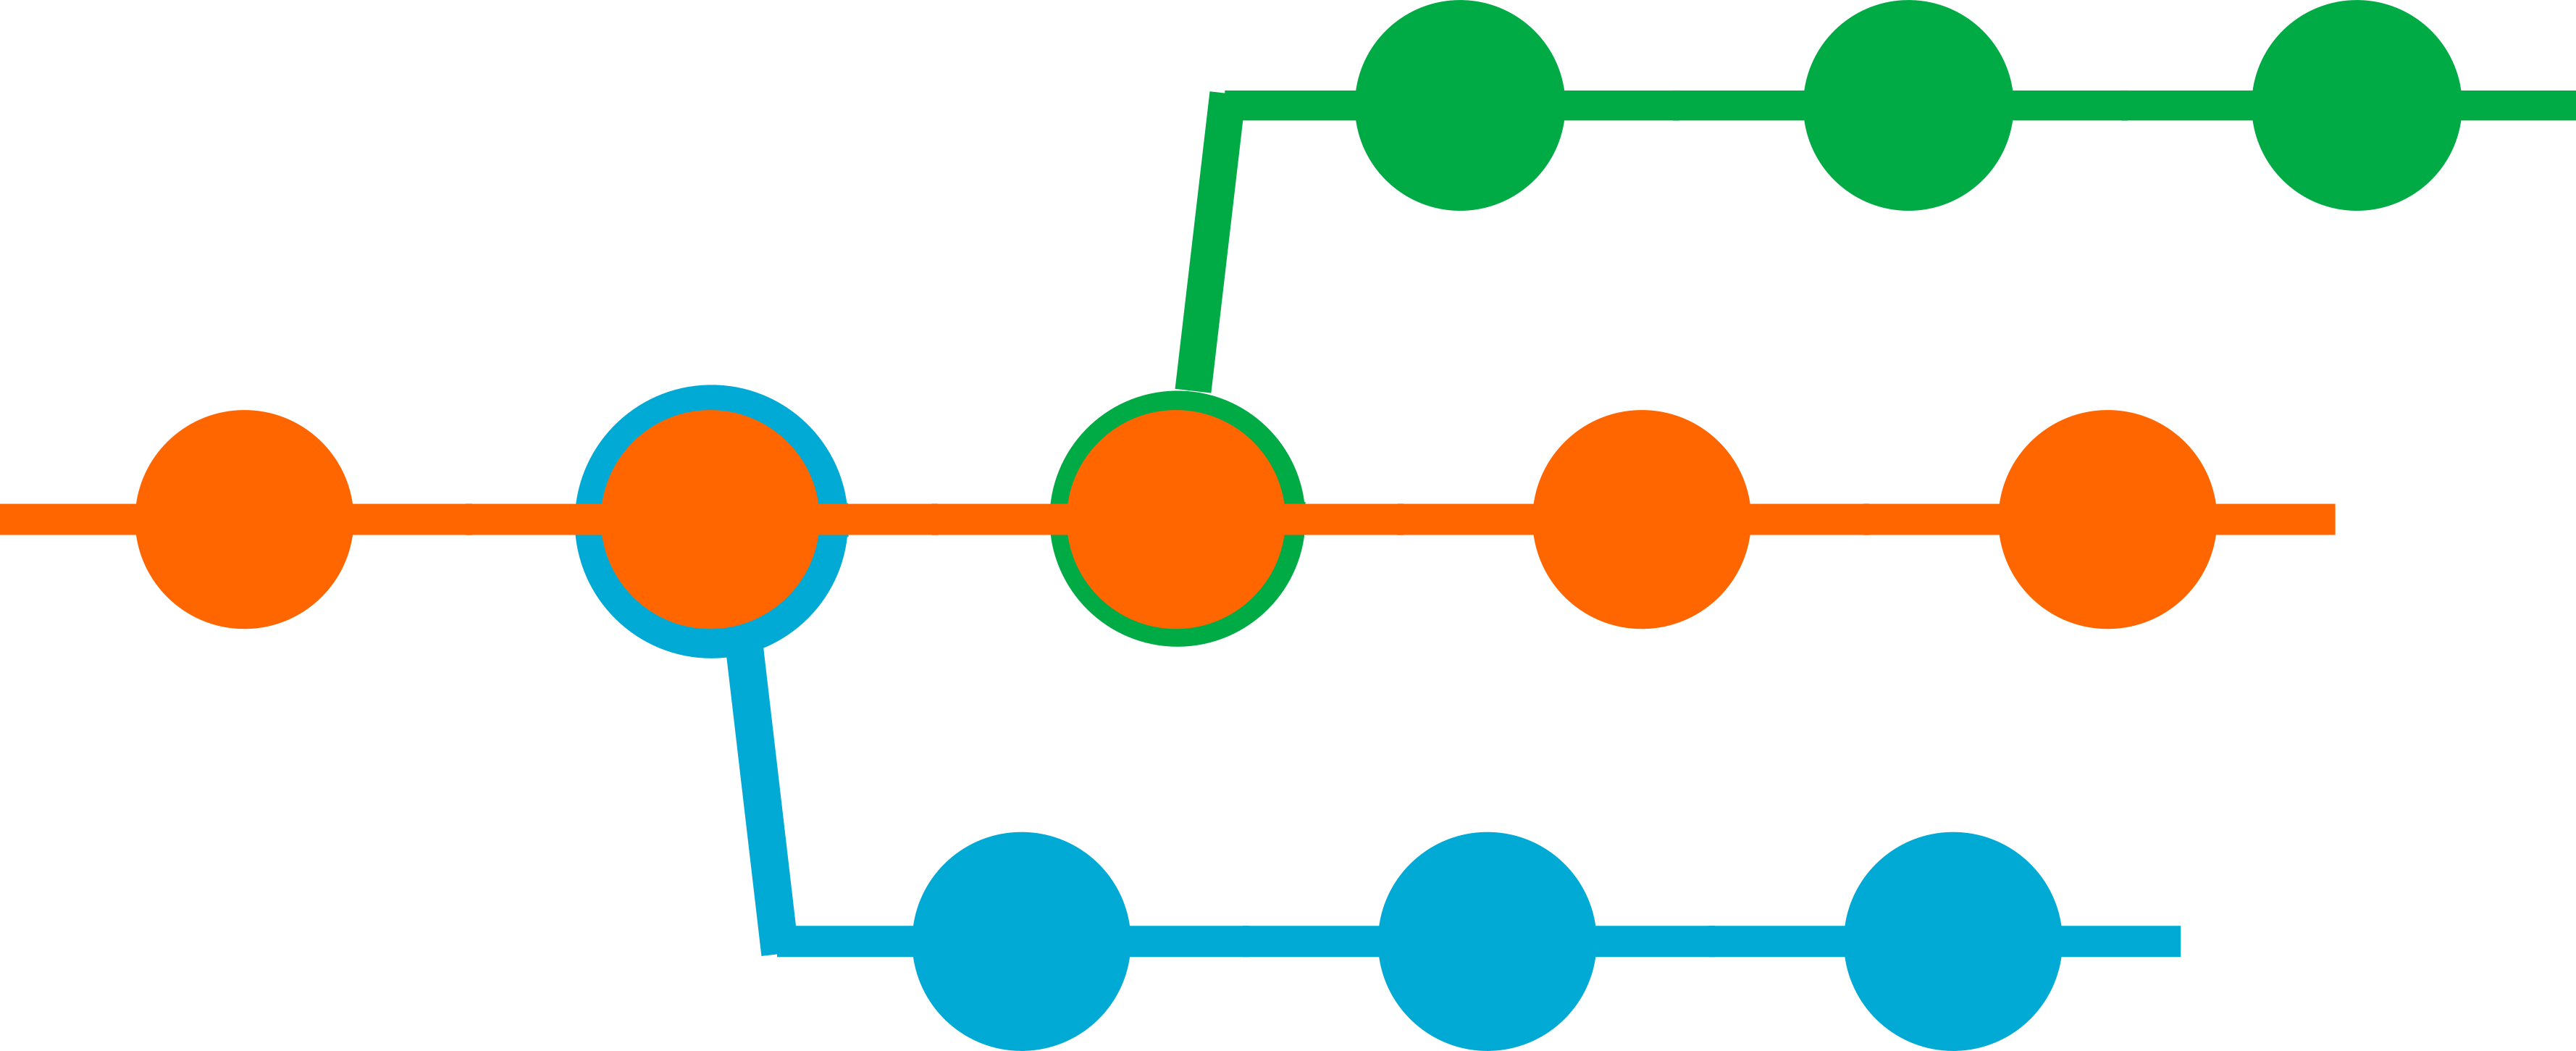
\includegraphics[width=9cm]{tree.png}
	\end{center}
	\end{frame}

	\begin{frame}{Terminology 2}
	\begin{description}
		\item[merge] merge two different branches together and keep chronological order
		\item[rebase] put a branch on top of another
		\item[pull] a shortcut for \textit{fetch} and \textit{merge}
		\item[conflict] a problem that blocks merging of changes
		\item[squash] put two (or more) commits into one
		\item[blame] display the author of a change
	\end{description}
	\end{frame}

	\begin{frame}{How does merging work?}
	\begin{center}
%		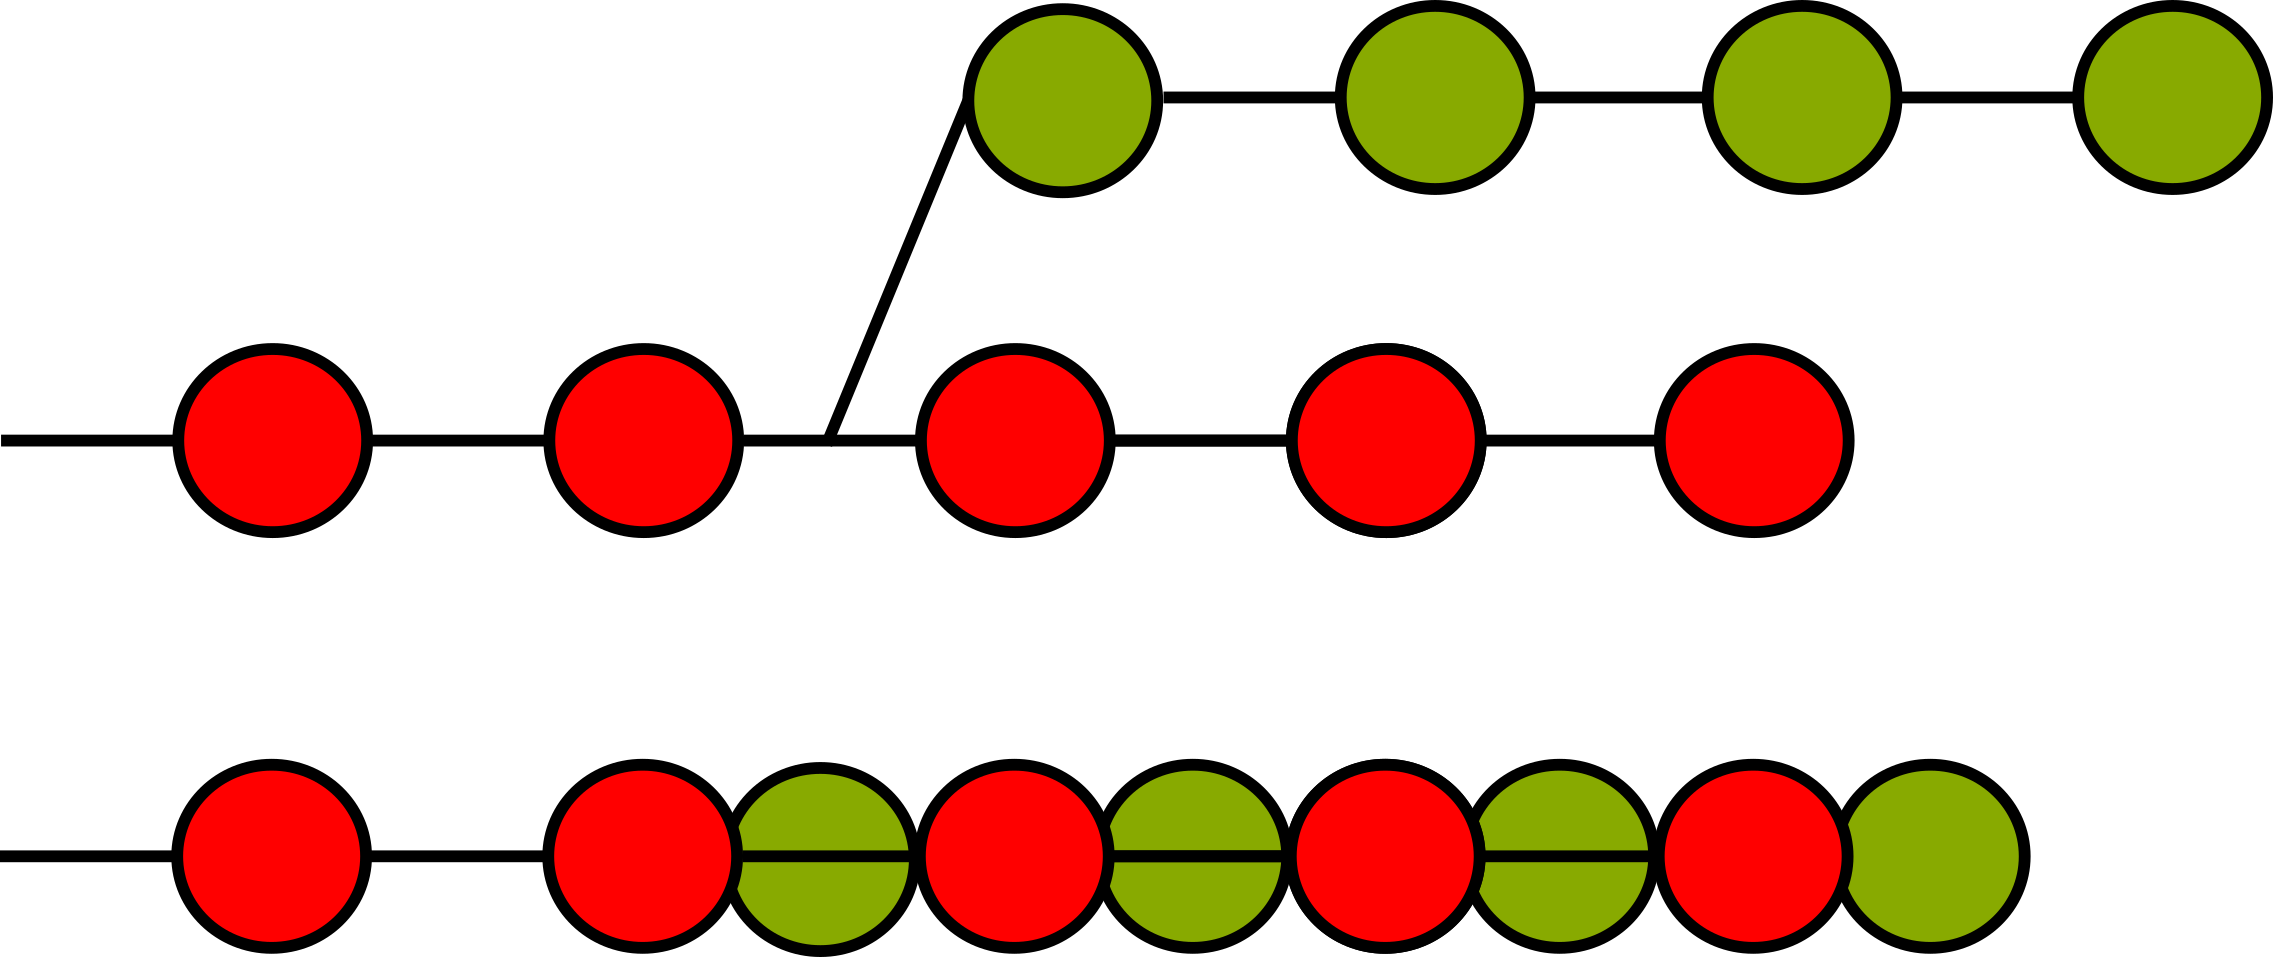
\includegraphics[width=9cm]{merge.png}
	\end{center}
	\end{frame}

	\begin{frame}{How does rebasing work?}
	\begin{center}
%		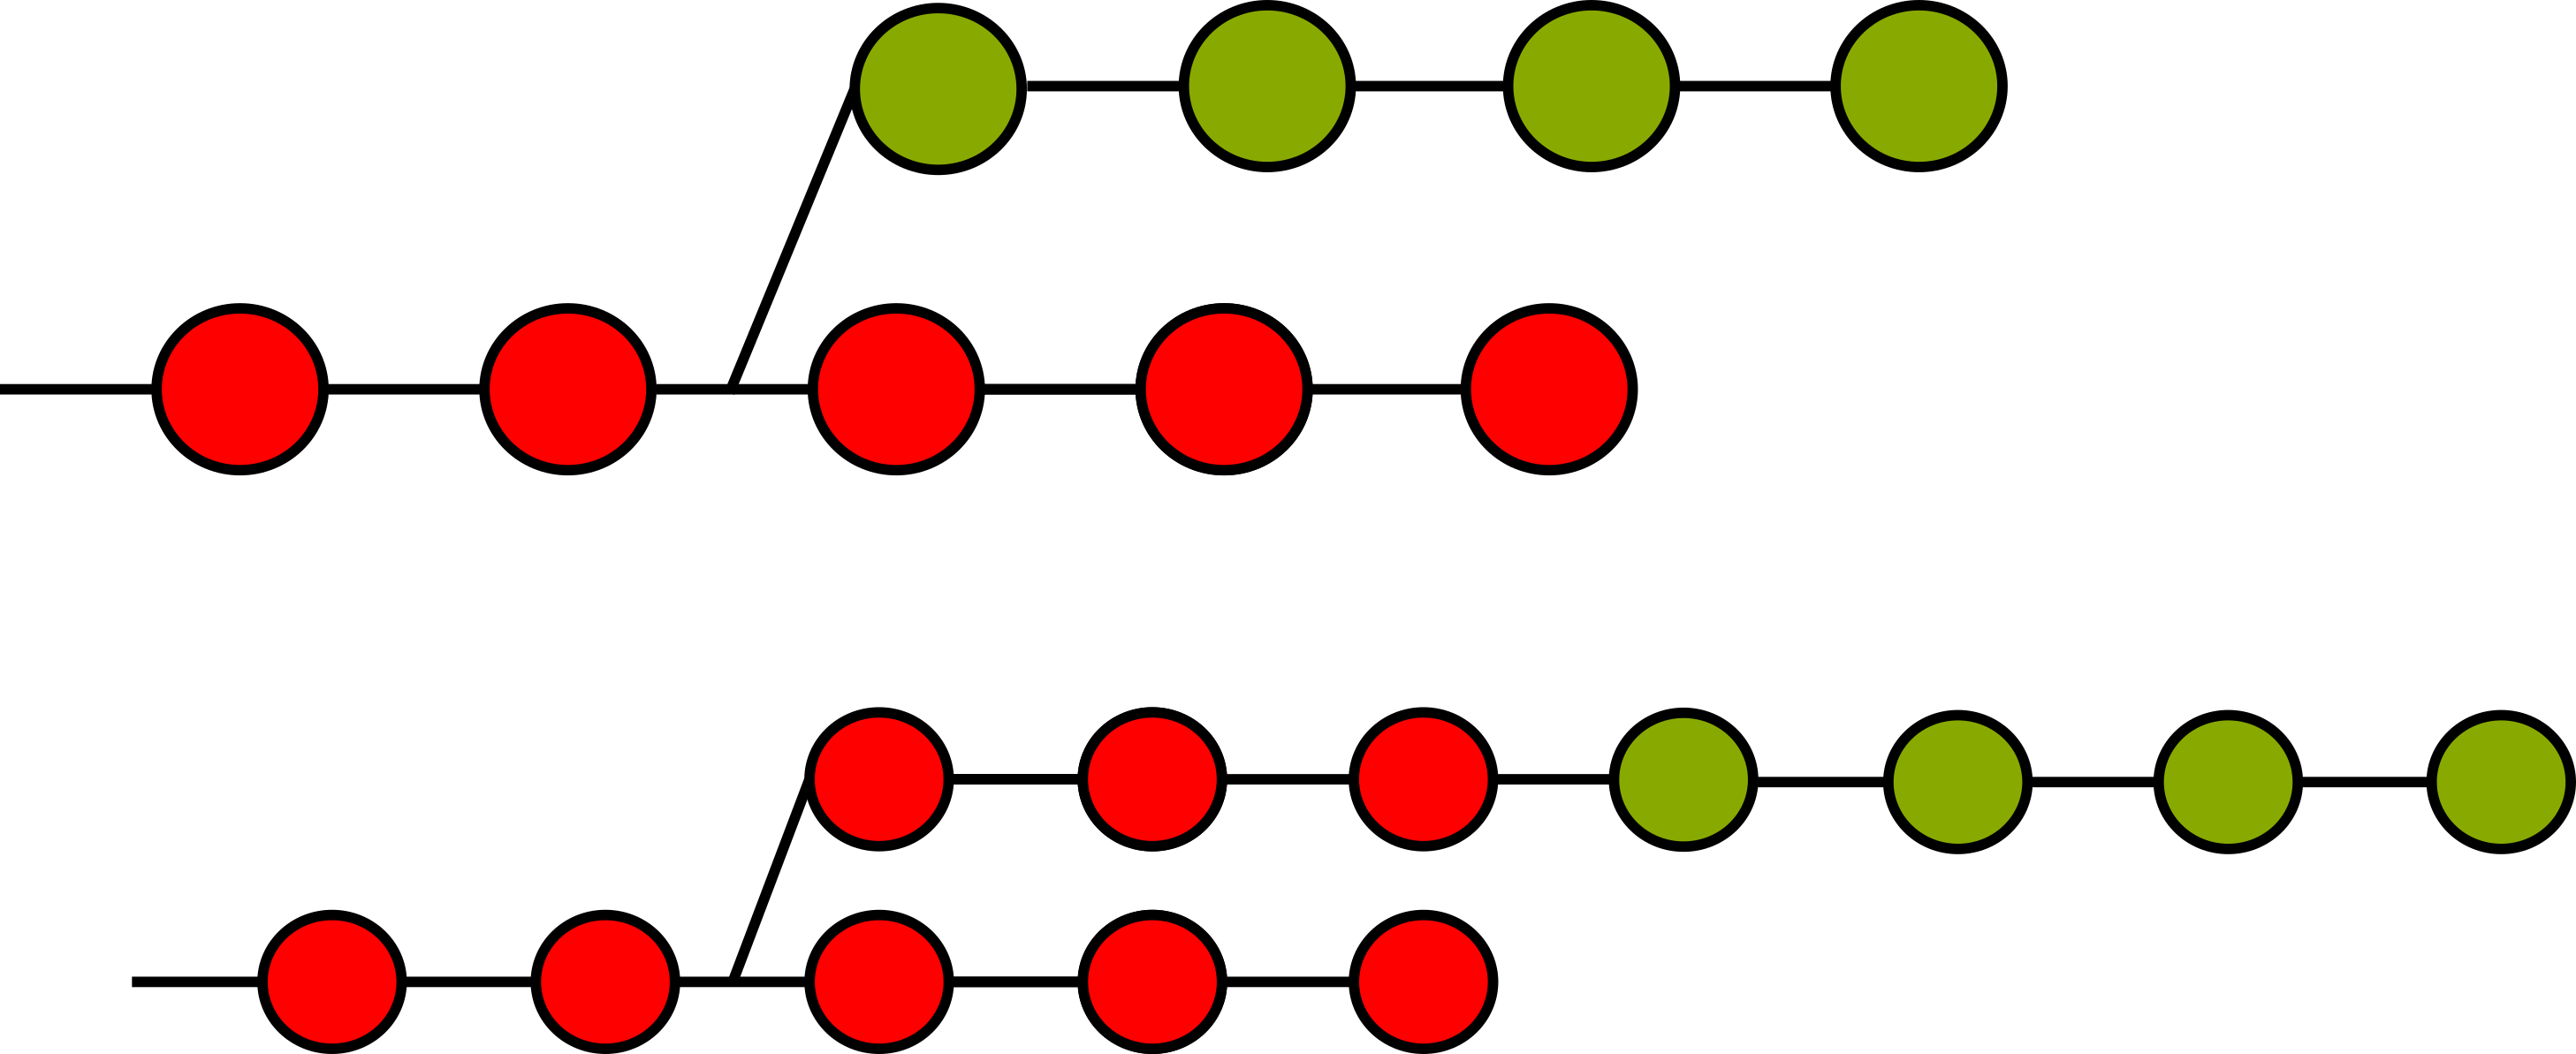
\includegraphics[width=9cm]{rebase.png}
	\end{center}
	\end{frame}

	\begin{frame}{Fork the repository}
	\begin{itemize}
		\item creates a server-based copy of the repo
		\item go to your Git forge webUI
		\item push the \textbf{Fork} button
	\end{itemize}
	\end{frame}


	\begin{frame}{Clone the repository}
	\begin{itemize}
		\item creates a local copy of the repository in a new directory
		\item \texttt{git clone <repo-address>}
		\item \texttt{git clone <repo-address> <directory>}
	\end{itemize}

	\end{frame}

	\begin{frame}{Task 1}
	\begin{enumerate}
		\item As a group, fork repository \\ {\small \url{https://github.com/dokumentarista/trygit.git}}.
		\item Set up commit rights for your members.
		\item Clone the fork to your machine.
		\item Go to that directory.
		\item Display its content (\texttt{ls -a})
	\end{enumerate}
	
	\end{frame}

	\begin{frame}{Developing the project (adding changes)}
		\begin{enumerate}
		\item open, edit, save files as you would normally do
		\item see the new status
	        \begin{itemize}
		    \item \texttt{git status}
	        \end{itemize}
		\item add files you want git to start tracking
	        \begin{itemize}
		    \item \texttt{git add}
	        \end{itemize}
		\item save the changed files into the git tree
	        \begin{itemize}
		    \item \texttt{git commit -m "Explain why"}
	        \end{itemize}
		\item synchronize your git tree with the server version
	        \begin{itemize}
		    \item \texttt{git push}
	        \end{itemize}
		\end{enumerate}
	\end{frame}

	\begin{frame}{Task 2}
	Although a group, work individually
	
	\vspace{5pt}

	    \begin{enumerate}
		\item Open the \texttt{names.txt} file in the repo
		\item Add your name to the list of names
		\item Commit your changes
		\item Push them onto the server
	    \end{enumerate}
	\end{frame}

	\begin{frame}{Getting the first conflict}
	Git conflict, sometimes referred to as \textbf{merge conflict}, happens when:
	
	\vspace{5pt}
	
	\begin{itemize}
		\item two (or more) versions of one change
		\item at the same time
	\end{itemize}

	\vspace{5pt}
	
	When in conflict, you cannot work with the remote repository because Git protects your data from being damaged.

\end{frame}

	\begin{frame}{When do I get a merge conflict?}
	\begin{center}
%		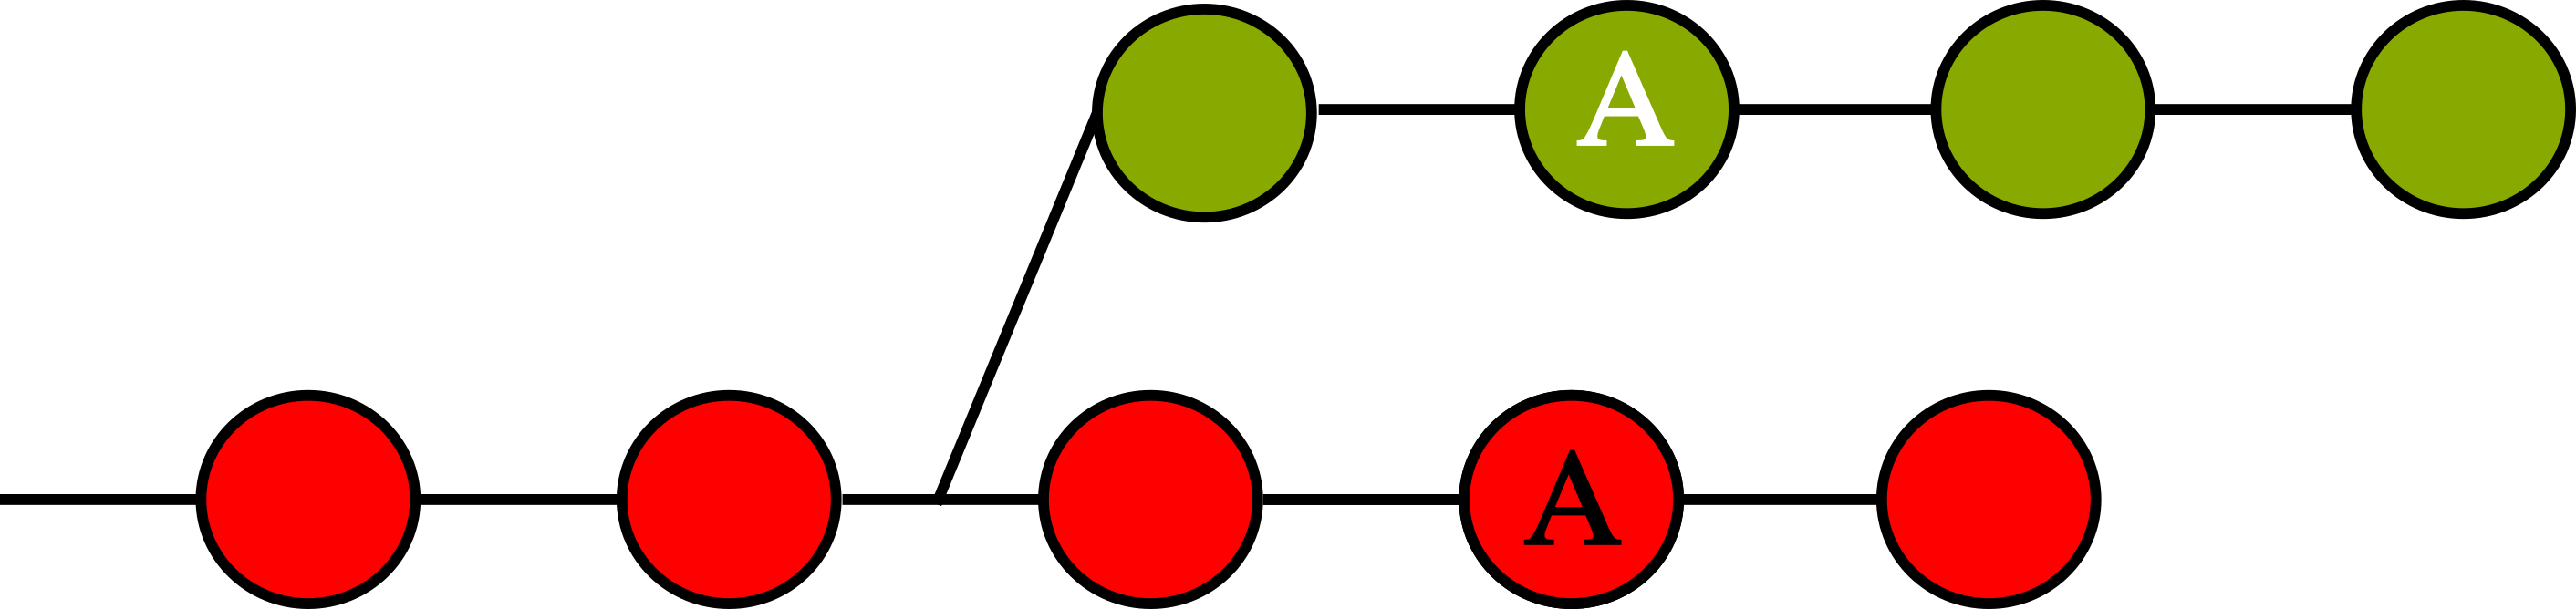
\includegraphics[width=9cm]{conflict.png}
	\end{center}
	\end{frame}


	\begin{frame}[fragile]{When you try to push}
	\begin{verbatim}
	 ! [rejected]        master -> master (fetch first)
	error: failed to push some refs to 
	'https://github.com/dokumentarista/trygit.git'
	hint: Updates were rejected because the remote 
	hint: contains work that you do
not have locally. 
	hint: This is usually caused by another repository 
	hint: pushing
to the same ref. You may want to first 
	hint: integrate the remote changes
(e.g., 'git pull ...')
	hint: before pushing again.
	hint: See the 'Note about fast-forwards' for details.
	\end{verbatim}
	\end{frame}

	\begin{frame}[fragile]{When you try to pull}
	\begin{verbatim}
	remote: Enumerating objects: 8, done.
	remote: Counting objects: 100% (8/8), done.
	remote: Compressing objects: 100% (6/6), done.
	remote: Total 6 (delta 2), reused 0 (delta 0) 
	Unpacking objects: 100% (6/6), done.
	From https://github.com/dokumentarista/trygit
	34c12d6..d8a0bea  master     -> origin/master
	Auto-merging names.md
	CONFLICT (content): Merge conflict in names.md
	Automatic merge failed; fix conflicts and then 
	commit the result.
	\end{verbatim}
\end{frame}

	\begin{frame}[fragile]{In the file}
	\begin{verbatim}
	# Names of login names.
	
	<<<<<<< HEAD                                                                                                           
	### Add your login name to the last available slot.
	
	1. pkratoch
	=======
	### Add your login name to the last available slot.
	
	1. lruzicka
	>>>>>>> d8a0beae9626d523d509b9fc53de06c435999d24
	2.
	3.
	4.
	5.
	\end{verbatim}
	\end{frame}

\begin{frame}{How to solve merge conflicts?}
	\begin{itemize}
		\item Open the conflicting file.
		\item Explore the marked area.
		\item Your changes are marked \textbf{HEAD} above the division line.
		\item \textbf{=======} is the division line.
		\item Remote changes are bellow the division line.
		\item Rewrite the file as you want it to be and save it.
		\item \texttt{git add corrected-file}.
		\item \texttt{git merge -\,-continue}
		\item Edit the commit message if asked.
	\end{itemize}
\end{frame}

	\begin{frame}[fragile]{Conflict fixed}
	\begin{verbatim}
	# Names of login names.
	
	### Add your login name to the last available slot.
	
	1. pkratoch
	2. lruzicka
	3.
	4.
	5.
	\end{verbatim}
	\end{frame}


	\begin{frame}{How to limit conflicts?}
	\begin{itemize}
		\item Work in \textbf{branches}.
		\item \textbf{Fork} the project and work in your version.
		\item Plan ahead.
		\item Communicate.
	\end{itemize}

	\vspace{5pt}

	Conflicts will always happen, love them, nurture them and fix them carefully.
\end{frame}

	\begin{frame}{What is a branch?}
	\begin{itemize}
		\item alternate development version
		\item it checks out from a certain commit
		\item it can branch from \textbf{master} or another branch
		\item it typically diverges from its origin very quickly
		\item it allows you to work individually without having to solve many conflicts as you go
	\end{itemize}
\end{frame}

	\begin{frame}{How to work in a branch?}
	\begin{itemize}
		\item Create a new branch (\texttt{git checkout -b new})
		\item Write your changes there.
		\item Fix merge conflicts if any.
		\item Merge or rebase possible changes in the original branch to your branch to make it merge ready.
		\item Have it merged (or rebased) back into its origin.
	\end{itemize}
\end{frame}

	\begin{frame}{git merge}
	\begin{itemize}
		\item Merges two branches into one.
		\item The checked-out branch will be altered.
		\item It keeps track of history.
		\item It is chronological.
		\item It produces a \textbf{merge message}
	\end{itemize}
\end{frame}

	\begin{frame}{git rebase}
	\begin{itemize}
		\item Merges two branches into one.
		\item The checked-out branch will be altered.
		\item It does not keep track of history.
		\item It is not chronological.
		\item It accepts foreign commits, merges them to your branch, and puts your commits on top of that.
		\item It helps to keep the history of the master branch free from merge commits.
	\end{itemize}
\end{frame}


	\begin{frame}{Task 3}
	\begin{enumerate}
		\item Delete the repo files and clone it again.
		\item Each person in the group creates their own branch.
		\item Communicate with the team.
		\item Add your name to the list of names in your branch.
		\item Merge or rebase the original branch onto your branch.
		\item Fix conflicts.
		\item Have it merged.
	\end{enumerate}
	\end{frame}

	\begin{frame}{Task 4}
	\begin{enumerate}
		\item As a group, fork repository \\ {\small \url{https://github.com/dokumentarista/crossword.git}}.
		\item Set up commit rights for your members.
		\item Clone the repo.
		\item Solve the crossword.
	\end{enumerate}
	
\end{frame}


	\begin{frame}{What if I don't have access to repository?}
	\begin{itemize}
		\item Very common in open source world
		\item Send patch via email?
	\end{itemize}
	\end{frame}

	\begin{frame}{Fork workflow}
	\begin{itemize}
		\item Fork a repository
		\item Clone a repository
	        \begin{itemize}
		    \item \texttt{git clone <repo-address> <directory>}
	        \end{itemize}
		\item See remote repositories
	        \begin{itemize}
		    \item \texttt{git remote -v}
	        \end{itemize}
		\item Add the other remote repository
	        \begin{itemize}
		    \item \texttt{git remote add <name> <repo-address>}
	        \end{itemize}
		\item Make changes and push them to your fork
	        \begin{itemize}
		    \item \texttt{git push --set-upstream <remote> <branch>}
	        \end{itemize}
		\item Make pull request
	\end{itemize}
	\end{frame}

	\begin{frame}{Changing the history -- interactive rebase}
	\begin{itemize}
		\item Can change commit messages.
		\item Can merge two (or more) commits -- squash them.
		\item Can throw away commits.
		\item Makes severe changes to the repo structure -- risky.
		\item It changes the fundaments for your collaborators.
		\item Needs to be force pushed.
		\item Should only be done in individual branches.
	\end{itemize}
\end{frame}

	\begin{frame}{How to recover from interactive rebase?}
	\begin{itemize}
		\item Checkout the branch.
		\item Fetch the new repo data 
		\begin{itemize}
			\item \texttt{git fetch origin}
		\end{itemize}
		\item Rebase your branch onto the original branch.
		\begin{itemize}
			\item \texttt{git rebase origin/master}
		\end{itemize}
		\item All changes from your branch will appear on top of the original branch.
		\item Alternatively, you can use an option that will do the rebase for you, if possible.
		\begin{itemize}
			\item \texttt{git pull -\,-rebase}
		\end{itemize}
		\item \textbf{Merging the branch would never work}, because the history has been changed.
	\end{itemize}
\end{frame}

\begin{frame}{Undo local changes -- reset}
	\begin{itemize}
		\item You can reset the HEAD to a previous commit.
		\item You can either use hashes or \texttt{HEAD$\sim$3}
		\item You can use \textbf{soft}, \textbf{mixed} or \textbf{hard} reset.
		\item Default is mixed -- it changes the HEAD marker and unstages files, but leaves them untouched.
		\item Hard reset will delete your files -- think twice.
		\item The operation goes back in history -- needs rebasing.
		\item All changes can be recovered until you push to the server.
		\item Should only be done in individual branches.
	\end{itemize}
\end{frame}

\begin{frame}{Undo local changes -- revert}
	\begin{itemize}
		\item You can revert to a previous commit.
		\item You can either use hashes or \texttt{HEAD$\sim$3}
		\item A new commit will be added, that undoes the changes.
		\item The operation does not go back in history, can be forwarded.
		\item All changes can be recovered any time locally.
		\item Can be done in cooperative branches.
	\end{itemize}
\end{frame}

\begin{frame}{Questions?}
	If you have any questions, just ask now \ldots{}
	
	\vspace{15pt}
	
	\ldots{} or hold it forever.
\end{frame}

\begin{frame}{}
	Thank you for your attention and have a great day!
\end{frame}



\end{document}
